% Created 2017-10-06 Fri 19:15
% Intended LaTeX compiler: pdflatex
\documentclass[11pt]{article}
\usepackage[utf8]{inputenc}
\usepackage[T1]{fontenc}
\usepackage{graphicx}
\usepackage{grffile}
\usepackage{longtable}
\usepackage{wrapfig}
\usepackage{rotating}
\usepackage[normalem]{ulem}
\usepackage{amsmath}
\usepackage{textcomp}
\usepackage{amssymb}
\usepackage{capt-of}
\usepackage{hyperref}
\usepackage{amsmath}
\author{Jake Brawer}
\date{\today}
\title{Assignment 4}
\hypersetup{
 pdfauthor={Jake Brawer},
 pdftitle={Assignment 4},
 pdfkeywords={},
 pdfsubject={},
 pdfcreator={Emacs 25.2.1 (Org mode 9.1.2)}, 
 pdflang={English}}
\begin{document}

\maketitle

\section*{Problem 1}
\label{sec:org69117b0}

\subsection*{(a)}
\label{sec:orgba514f3}

\begin{align}
  F_{x}(X) &= P\left\{X \leq x\}\right\\ 
       &= P\left\{s\tan{A} + \theta \leq x\}\right\\
       &=P\left\{A \leq \arctan{\frac{x-\theta}{s}}\right\}\\
       &=(\arctan{\frac{x-\theta}{s} + \frac{\pi}{2})\frac{1}{\pi}}\\
\end{align}

So:\\
\begin{align}
F_{x}'(X) &= \frac{1}{s \pi (1 + \frac{x - \theta}{s})}\\
          &=\frac{1}{s}\kappa(\frac{x-\theta}{s})\\
          &= f_{x}
\end{align}

\subsection*{(b)}
\label{sec:org279f2ee}

\begin{verbatim}
Ths <- seq(-30, 10, 0.2)
Ss <- seq(.2, 40, .2)

Xs <- c(1,2,7.8,9.2)

likefcn <- function(th, s){
  return(prod(1/(pi*s*(1.0+((Xs-th) / s)^2))))
}

m <- length(Ss)
n <- length(Ths)
liks <- matrix(0, nrow=m, ncol=n)
for(i in 1:m){
  for(j in 1:n){
    liks[i, j] = likefcn(Ths[j], Ss[i])
  }
}
length(liks)
\end{verbatim}

\begin{verbatim}
40200
\end{verbatim}


\subsection*{(c)}
\label{sec:org7026247}

\begin{verbatim}
persp(Ss,Ths, liks, theta=30, phi=30, expand=0.5, 
col="lightblue", zlab="z=f(x,y)",  
ticktype="detailed", 
shade=.75, lphi=45, ltheta=135)
\end{verbatim}

\begin{center}
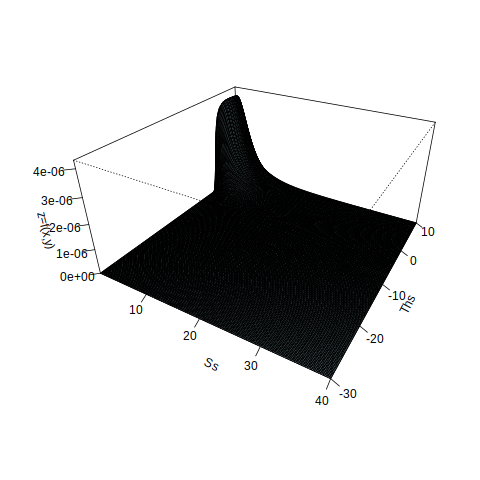
\includegraphics[width=.9\linewidth]{3d.png}
\end{center}


Sorry this is all I had time to do ;\_; 
\end{document}